\section{SafeDE: a \underline{D}iversity \underline{E}nforcement hardware module}
\label{sec:dimmo}

This section presents SafeDE. First, we introduce the architecture of SafeDE. Then, we analyze its pros and cons in comparison with the software-only solution. Finally, we provide implementation and integration details about its deployment in a commercial space multicore.

\subsection{SafeDE Architecture}

\begin{figure}[t!]
\centering
  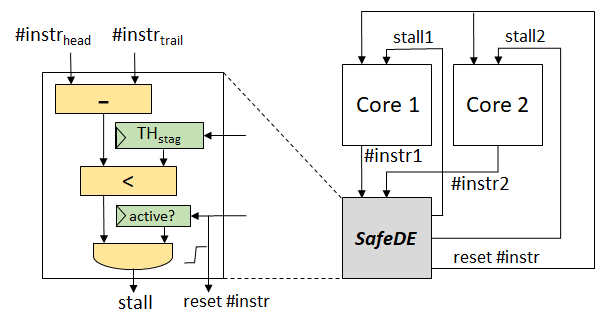
\includegraphics[width=1\columnwidth]{imgs/dimmo.png} 
  \caption{SafeDE architecture.}
  \label{fig:dimmo}
\end{figure}

SafeDE is architected to be the hardware counterpart of software-based light lockstepping. Its objective is keeping as much as possible the advantages of the software-only solution, while mitigating its limitations, which we discuss in next subsection. For that purpose, SafeDE is devised as a tiny module coupled to each pair of cores potentially needing to operate lockstepped. This is illustrated in Figure~\ref{fig:dimmo}. As shown, SafeDE requires the instruction count values of the lockstepped cores, as well as an interface signal to stall the trail core. SafeDE subtracts the number of instructions of the trail core from those of the head core, $\#instr_{head} - \#instr_{trail}$, as in the case of the software-only solution, and compares the difference against a staggering threshold, $TH_{stag}$. Only when the head core is not sufficiently ahead of the trail core, and SafeDE is active, a stall signal is sent to the trail core, which must be used to stall the core whenever set. Such stall can be achieved, for instance, stalling all stages (e.g. blocking pipeline latches), stalling only the commit stage, or stalling only the fetch stage, to name few alternatives. 

\textbf{SafeDE parameters}. SafeDE has four configuration registers: $TH_{stag}$, $active$, $CritSec1$ and $CritSec2$. 
%\textcolor{red}{SA: Later on we describre that we use 3 registers}
\begin{itemize}
\item $TH_{stag}$ stands for the minimum number of instructions that the head core must be ahead of the trail core. Typical values are few instructions, very much in line with hardware-based tight lockstepped cores. Note that this value is several orders of magnitude lower than that for software-only solutions. 
\item $active$ signal indicates whether SafeDE is active or not. If reset, SafeDE produces no effect. Else, SafeDE operates normally. Whenever the parameter is set to 1 (input signal raised), lockstep operation is possible, which is practically controlled by the other registers.
\item $CritSec1$ and $CritSec2$ registers indicate whether core 1 (head) and core 2 (trail) have entered the ``critical'' code region to be executed in lockstep mode. 
%a reset signal is sent to $\#instr_{head}$ and $\#instr_{trail}$ so that they are reset synchronizedly.
\end{itemize}

\textbf{SafeDE operation}. SafeDE is, at some point, inactive ($active=0$). No action is performed by SafeDE until $active$ is set, regardless of the values of the other registers. 
Eventually, SafeDE is programmed setting $TH_{stag}$ as needed, and then $active$ is set.
Once $active=1$, $CritSec1$ and $CritSec2$ are reset, and SafeDE awaits for the corresponding activation of $CritSec1$ and $CritSec2$.  
$CritSec1$ and $CritSec2$ are set by core1 and core2 respectively when they reach their critical section. The first core entering the critical section will take the role of the head core. Whenever the head core sets its $CritSec$ register, its instruction count ($\#instr_{head}$) resets and starts counting the committed instructions. If the trail core activates its $CritSec$ register before the staggering is large enough ($\#instr_{head} - \#instr_{trail} < TH_{stag}$), the stall signal is sent to the trail core.
%Whenever $CritSec1$ is set, the head core gets its instruction count reset ($\#instr_{head}$) and executes normally. Whenever $CritSec2$ is set, the trail core gets its instruction count reset ($\#instr_{trail}$) and waits for (1) the head core to enter its critical code region ($CritSec1$ is set), and (2) for the staggering to be large enough. If $CritSec1$ is not set, or $\#instr_{head} - \#instr_{trail} < TH_{stag}$, then a stall signal is sent to the trail core.
%Since the stall signal for the trail core is ANDed with $active$, it is zero and no action is performed. 
%Whenever $active$ is set, $\#instr_{head}$ and $\#instr_{trail}$ in the head and trail cores respectively are reset. 
%Then, if SafeDE detects that the $\#instr_{head} - \#instr_{trail} < TH_{stag}$, then a stall signal is sent to the trail core. 
%Note that this occurs automatically when SafeDE is activated since $\#instr_{head}$ and $\#instr_{trail}$ are both reset simultaneously. 
%This allows the head core to gain some staggering w.r.t. the trail core. 
As soon as the staggering is enough, the stall signal is reset and the trail core starts execution. Note that SafeDE performs the subtraction $\#instr_{head} - \#instr_{trail}$ and the comparison against $TH_{stag}$ every cycle. This allows using very low values for $TH_{stag}$ as opposed to the software-only solution. Despite performing such action every cycle, note that $\#instr_{head}$ and $\#instr_{trail}$ barely change every cycle (e.g. they do not change or just are incremented by up to very few instructions). Therefore, activity due to the subtraction and comparison is tiny since most of input signals remain constant, and hence, signal switching occurs seldom.
Whenever the head core reaches the end of its critical section, it resets $CritSec1$. From that point onwards, SafeDE allows the trail core execute without any stall until it also finishes its critical region ($CritSec2$ is also reset).


\textbf{Software process}. To use SafeDE, end users, either by themselves or with the support from an appropriate API, need to create the two redundant processes, schedule them to the head and trail cores, and keep them stopped (e.g. with $SIG\_STOP$ signals). Then, SafeDE needs being configured and set to active state. Finally, both redundant processes need to be set to active (e.g. with $SIG\_CONT$ signals).


\subsection{Features and Limitations Analysis}

SafeDE offers a different tradeoff to that of the software-only solution. Next, we detail its main features and limitations along with whether they are common with the software-only solution in \cite{SergiDFT} or not.

\subsubsection{SafeDE features}
\begin{itemize}
\item \textbf{Low cost}. As shown before, SafeDE is a tiny module offering support to enforce staggering to achieve diverse redundancy. SafeDE releases the system from having to allocate a task with strict timing requirements (e.g. executing at a very specific frequency), as needed in the case of the software-only solution. 
\item \textbf{Low staggering}. By being implemented in hardware and monitoring instruction counts from the head and trail cores constantly, SafeDE can guarantee diversity even if staggering is low (e.g. $TH_{stag}$ set to few instructions). This is also an advantage w.r.t. the software-only solution, which requires heavier activities by being conducted by software means, reading remote registers, issuing interrupts to stall/resume execution in a core, etc., so needing a much higher staggering than SafeDE.
\item \textbf{Flexibility}. SafeDE can be enabled/disabled at will, thus being usable at very fine granularity. Still, the granularity is dictated by the ability of the software to create the redundant processes and stop/resume them at start up. Hence, flexibility is high, but the granularity at which SafeDE can be used is similar to that of the software-only solution.
\item \textbf{Low intrusiveness}. SafeDE needs cores to export few signals for its integration, thus being much less intrusive than hardware-based tight lockstepping. In particular, SafeDE needs cores to expose their instruction count register for monitoring purposes, an appropriate stall signal to stall the trail core whenever needed, and the reset signal for the instruction count register. 
%Thus, these are minor changes to the cores. 
Differently, the software-only solution does not require any hardware change, although it may require modifications into the operating system to allow reading the instruction count register from remote cores. SafeDE, instead, does not need any such operating system change.
\end{itemize}

\subsubsection{SafeDE limitations}
\begin{itemize}
\item \textbf{Non-null intrusiveness}. Hardware changes required by SafeDE are minor, but they are not null, so differently to the software-only solution, SafeDE cannot be deployed on COTS ASIC multicores.
\item \textbf{Limited applicability}. SafeDE, as well as the software-only solution, needs that redundant processes execute exactly the same instructions so that software does not diverge. Otherwise, SafeDE (and the software solution) would become ineffective. For instance, this implies that SafeDE should not be used for functions whose execution path depends on random choices or physical address bits, which could follow different paths across redundant processes. For the former case, SafeDE can be used if identical random values are enforced across processes (e.g. providing the same random number stream with a software-implemented pseudo-random number generator initialized identically for both processes). Similarly, SafeDE cannot be used for parallel applications if the execution path and the instruction count may vary across redundant threads due to synchronization (e.g. different order to access sequential code regions). In any case, such limitation is analogous to that of the software-only solution. Also, SafeDE (and software solutions) cannot be applied for processes with some form of I/O accesses, since those accesses need to be performed only once generally, but redundant processes would perform those accesses twice.
\item \textbf{Limited diversity}. Physical diversity is achieved by running redundant processes in different cores. SafeDE, as well as the software only solution, provides also time diversity. However, other sources of \emph{common cause failures} (i.e. identical failures in both cores due to a single fault), such as for instance those related to physical degradation of specific gates of the processor need other types of diversity (e.g. layout diversity) that cannot be achieved by any external monitor, either hardware (SafeDE) or software.
\item \textbf{SafeDE hardening}. Since faults could also affect SafeDE, it must be hardened to meet sufficiently low failure rates or, simply, deployed with physical diverse redundancy, as for tight lockstepped cores (e.g. using the scheme in Figure~\ref{fig:HWSWlockstep}(a) but for SafeDE instead of the cores). 
\end{itemize}

\subsubsection{Scope of applicability}
Due to the limited applicability of SafeDE, as in the case of software-only solutions, SafeDE cannot be applied to all software but to code regions. For instance, if data is read from a sensor, processed and sent to an actuator, SafeDE and software only solutions can be applied to the processing part only. If full (end-to-end) diverse redundancy is needed, native (hardware-based) tight lockstepping support is needed, as explained in \cite{SergiDFT}. In particular, at least two cores need to be paired with hardware-based tight lockstepping to execute sensor and actuator interactions. However, the most performance hungry part of the execution (i.e. data processing) can be managed with SafeDE. Thus, deployments where only two cores provide hardware-based tight lockstepping, and the rest support light lockstepping with SafeDE would be highly efficient. For instance, an 8-core multicore could be deployed with (a) 4 pairs of hardware-based tight lockstepped cores, thus offering only 4 user-visible cores; (b) 1 pair of hardware-based tight lockstepped cores and 6 non-lockstepped cores, thus offering 7 user-visible cores, but only up to 1 concurrent task running with diverse redundancy; or (c) 1 pair of hardware-based tight lockstepped cores and 6 cores paired with SafeDE, thus offering 7 user-visible cores, and supporting up to 4 concurrent tasks running with diverse redundancy. 
%While other hybrid combinations would be possible (e.g. 2 pairs of hardware-based tight lockstepped cores and 4 non-lockstepped cores), examples (a), (b) and (c) already allow understanding the flexibility offered by SafeDE.



\subsection{Implementation and Integration}
\label{sec:integ}

\begin{figure}[t!]
\centering
  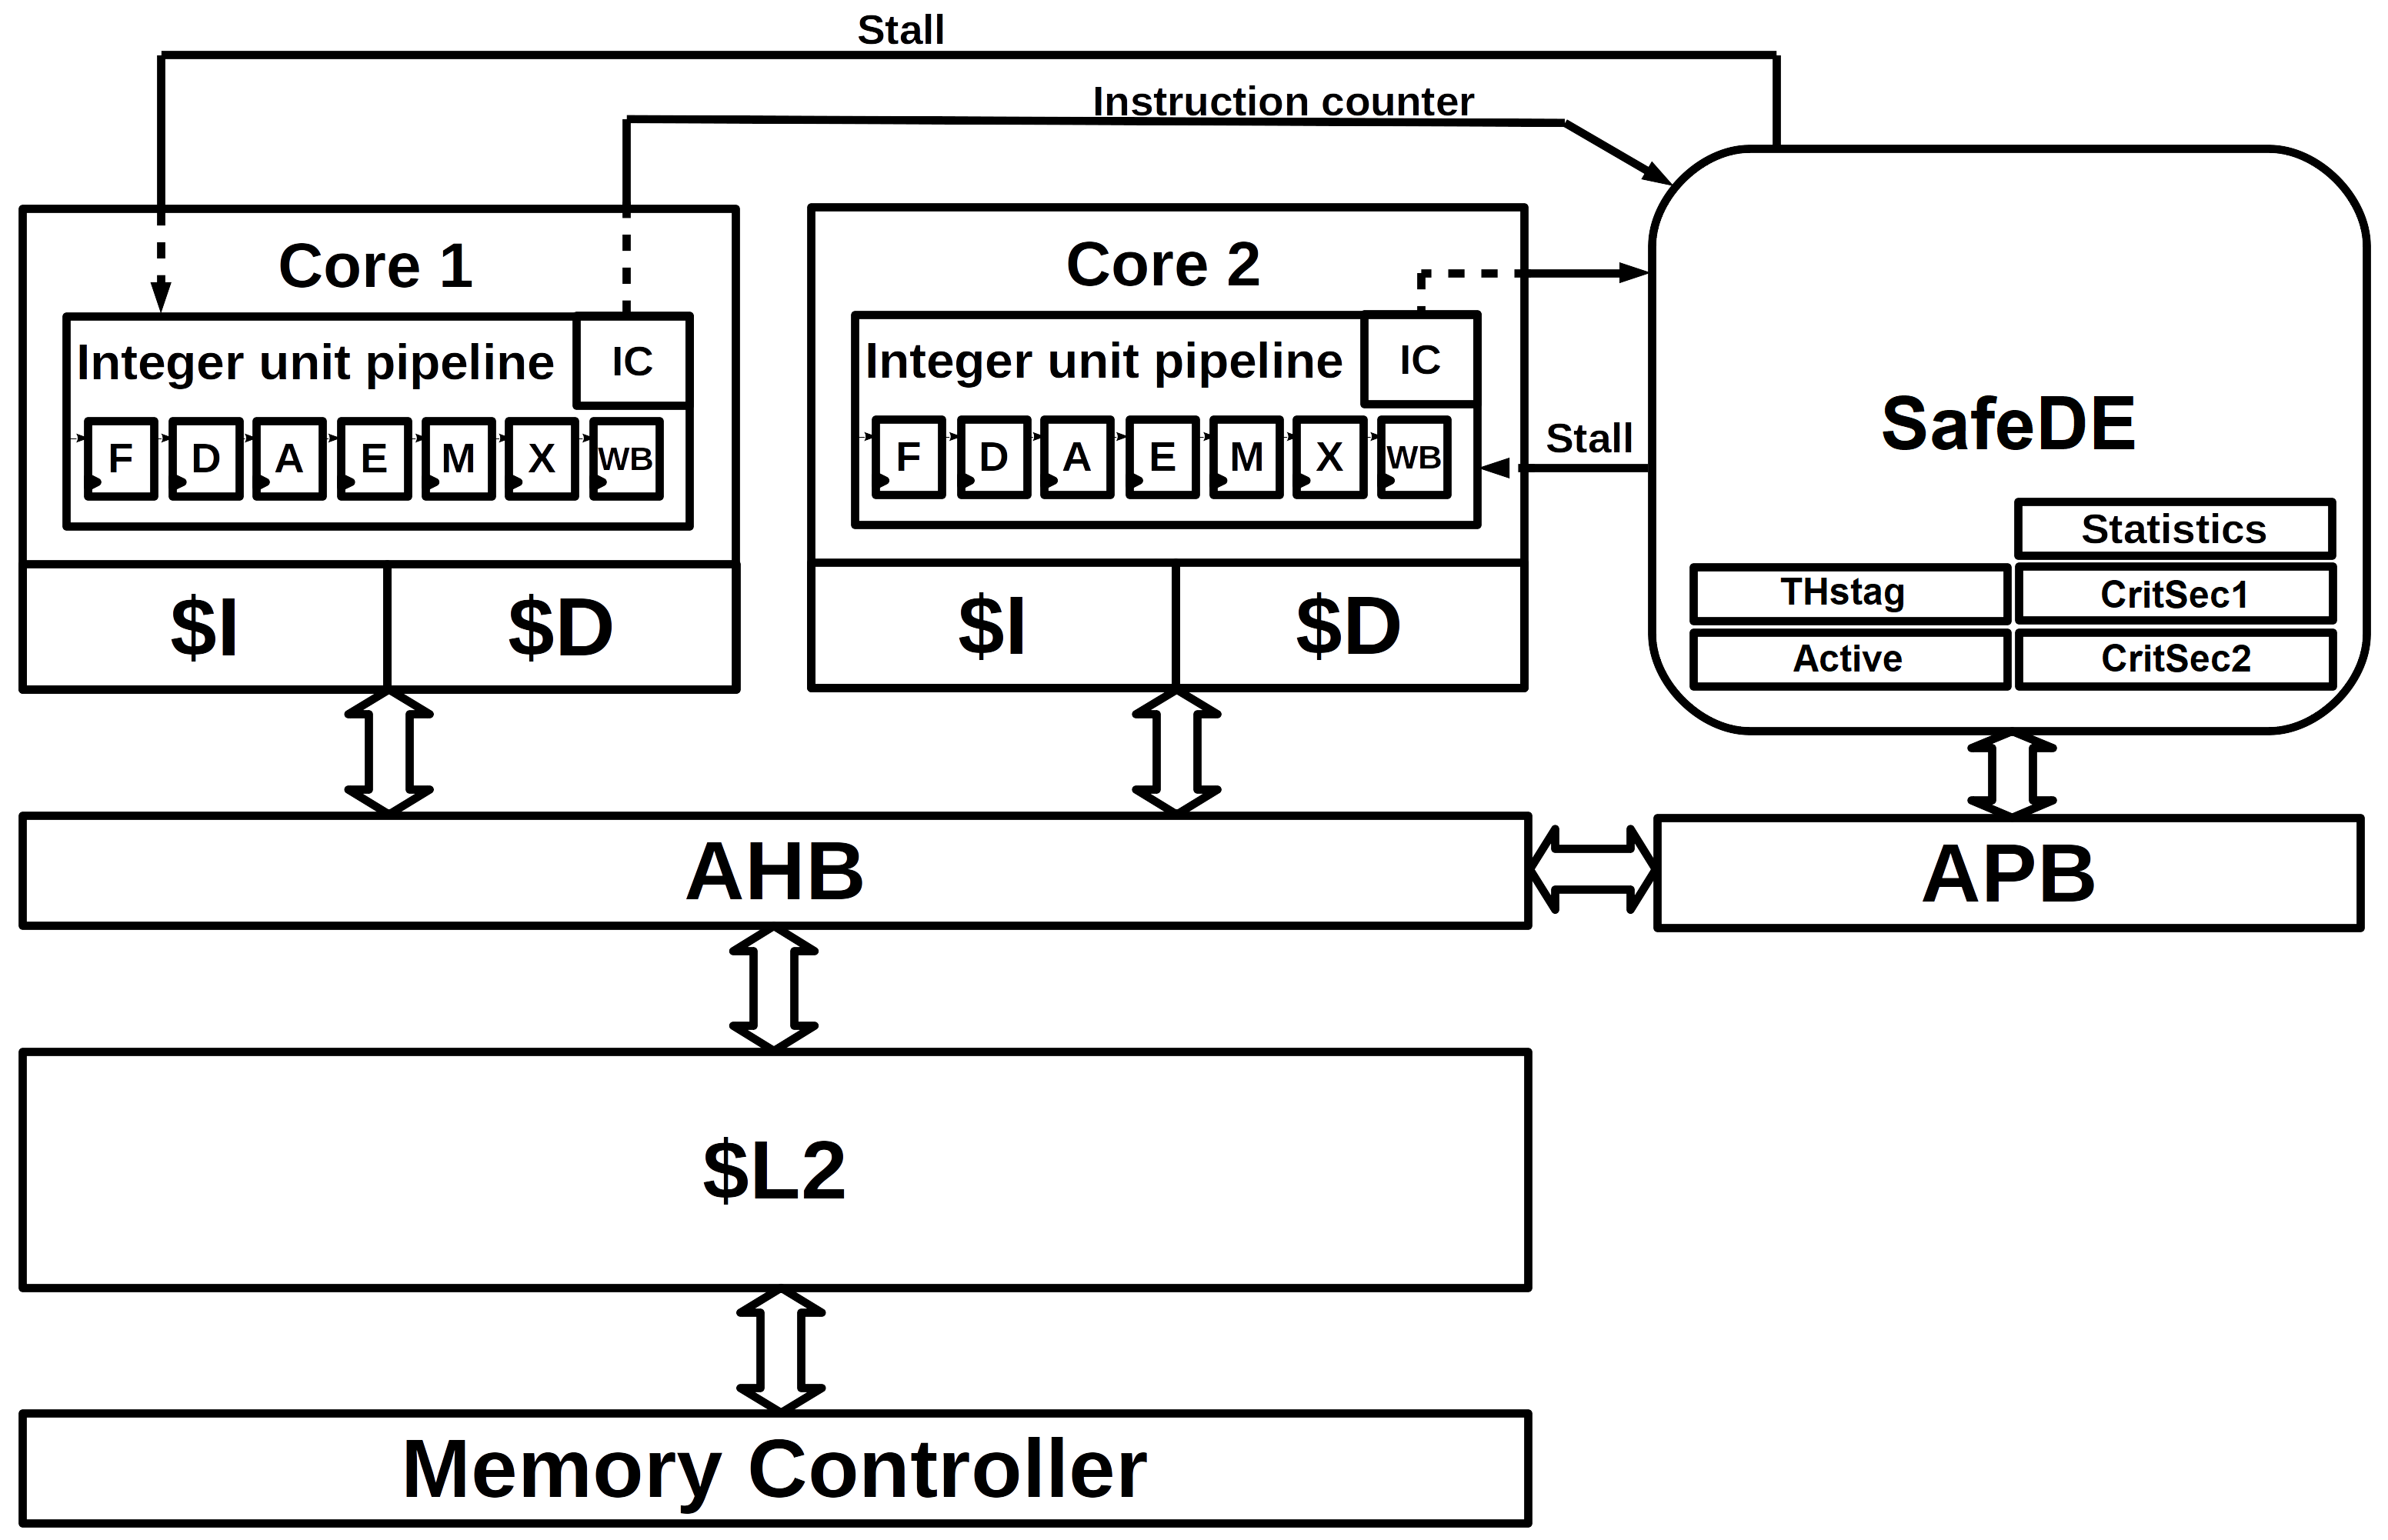
\includegraphics[width=1\columnwidth]{imgs/system.png} 
  \caption{High-level representation of SafeDE integrated into the system.}
  \label{fig:system}
\end{figure}

To prove its feasibility, SafeDE has been integrated and evaluated in an industrial space product, namely the RISC-V based Cobham Gaisler NOEL-V MultiProcessor System on Chip (MPSoC). In this platform, Cobham Gaisler provides an integrated set of reusable VHDL IP cores centered around common on-chip buses. The buses of the selected MPSoC are based on the standard AMBA 2.0. SafeDE is designed in VHDL as one of the reusable Gaisler IP cores. 

\subsubsection{System on Chip}
The SoC where SafeDE is tested comprises 2 RISC-V based 64-bit dual-issue 7-stages pipeline NOEL-V cores. Apart from the main 128 bits Advanced High-performance Bus (AHB), another AHB is used for debugging purposes. For low bandwidth peripherals as SafeDE, an Advanced Peripheral Bus (APB) is employed.

Each core includes private L1 Data and Instruction caches. Data L1 caches are write-through with a write-no-allocate policy. A shared L2 cache is connected to the main shared AMBA AHB, and to the memory controller. 


\subsubsection{Integration}
SafeDE is integrated as an APB slave connected to the system through a standard APB interface. Thus, SafeDE is highly portable and can be easily embedded into any system implementing an APB interface.

Apart from the APB standard signals, SafeDE needs a few interconnections with the cores. The instruction counter of each core has to be mapped as an input. Instruction counters are employed to calculate the total number of instructions commited by each core and compute its difference. SafeDE has one output to stall the trail core. That SafeDE output is ORed with an internal pipeline signal in charge of holding the pipeline (i.e. keeping constant the pipeline registers values). Therefore, when SafeDE needs to stall the trail core, SafeDE can stall that core just asserting the respective output. 
Therefore, the only modifications needed in the cores correspond to exporting the instruction counter\footnote{Note that virtually any processor implements instruction and cycle performance monitoring counters.} value to make it visible to SafeDE, and placing the OR gate needed let SafeDE set the pipeline stall signal whenever needed.
Figure \ref{fig:system} shows a high-level representation of SafeDE integrated into the system.


\subsubsection{Configuration and operation}
SafeDE is controlled and configured by means of four internal registers. Each register is mapped to a specific SoC memory position. The first one, $TH_{stag}$, is used to configure the minimum staggering. The second one, $active$, is used to enable/disable SafeDE. Each of the two remaining registers, $CritSec1$ and $CritSec2$, is coupled with one core and set to 1 when the respective core starts the critical section (i.e. with a store instruction to this register in the application), and set to 0 when it finishes its execution. This procedure allows SafeDE to synchronize both cores at the beginning of the critical section, even if they do not start simultaneously, as explained before. Neither of the cores assumes the role of trail or head core until its critical section starts. 
%The first core writing its SafeDE enable register is set as the head core during that execution.

%A detection mechanism was also designed to ensure that both cores reach the critical section within a specified time. Otherwise, an interruption is raised.

In addition to these four registers, SafeDE has also several registers to gather some statistics such as maximum staggering, minimum staggering, times that the trail core has been stalled, how many cycles the trail core has been stalled, committed instructions by each core, etc. The connection of SafeDE to the MPSoC allows SafeDE registers to be written and read through usual load and store operations. 

